% =============================================================================
% OpenMC-Metal: Monte Carlo Neutron Transport on Apple Metal GPU
% arXiv preprint
% =============================================================================
\documentclass[preprint,12pt]{elsarticle}

\usepackage{amsmath,amssymb}
\usepackage{graphicx}
\usepackage{booktabs}
\usepackage{siunitx}
\usepackage{hyperref}
\usepackage{xcolor}
\usepackage{algorithm}
\usepackage{algpseudocode}
\usepackage{tikz}
\usetikzlibrary{shapes.geometric, arrows.meta, positioning, fit, calc}

\hypersetup{
    colorlinks=true,
    linkcolor=blue!70!black,
    citecolor=blue!70!black,
    urlcolor=blue!70!black
}

\journal{Annals of Nuclear Energy}

\begin{document}

\begin{frontmatter}

\title{Monte Carlo Neutron Transport on Apple Metal GPU:\\
From Event-Based Kernel Fusion to History-Based Persistent Transport}

\author[anthropic]{Claude\fnref{fn_ai}}
\author[kaeri]{Yonggyun Yu\corref{cor1}}
\ead{ygyu@kaeri.re.kr}
\cortext[cor1]{Corresponding author}
\fntext[fn_ai]{AI assistant (Anthropic). Contributed to code implementation, data analysis, and manuscript preparation.}
\address[anthropic]{Anthropic, San Francisco, CA, USA}
\address[kaeri]{Korea Atomic Energy Research Institute (KAERI),
Daejeon 34057, Republic of Korea}

\begin{abstract}
We present the first implementation of Monte Carlo (MC) neutron transport
on Apple Silicon using the Metal GPU compute framework, exploring two
GPU transport architectures.
An event-based design with three fused kernels per transport step
achieves \num{112000}~histories/sec for the C5G7 seven-group
17$\times$17 assembly benchmark, matching a single NVIDIA V100 running
MC/DC (\num{109000}~histories/sec)---a hardware-only comparison using
the same algorithm class.
A history-based persistent kernel---where each GPU thread runs an
entire particle lifetime in a single dispatch---achieves
\num{1776000}~histories/sec on the same hardware, a $15.9\times$
speedup over the event-based design.  This improvement is primarily
algorithmic (eliminating ${\sim}600$ kernel dispatches per batch) and
would likely transfer to other GPU platforms.
Throughput scales to \num{3370000}~histories/sec at
\num{100000000}~particles for the pincell geometry.
At \SI{40}{\watt} thermal design power versus \SI{300}{\watt} for
the V100, the event-based architecture delivers $7.7\times$ better
energy efficiency (\num{2794} vs.\ \num{363}~histories/sec/W),
reflecting Apple Silicon's unified memory and SoC integration
advantages.
The pincell eigenvalue converges to $k_\mathrm{eff} = 1.3254 \pm
0.0004$ (reference: 1.3301, $\Delta = -470$~pcm), validating
transport physics across both architectures.
The implementation uses Python with PyObjC Metal bindings, requiring
no CUDA toolchain and running on consumer hardware.
\end{abstract}

\begin{keyword}
Monte Carlo \sep neutron transport \sep GPU computing \sep
Apple Metal \sep Apple Silicon \sep energy efficiency \sep C5G7 benchmark
\end{keyword}

\end{frontmatter}

% =============================================================================
\section{Introduction}
\label{sec:introduction}
% =============================================================================

Monte Carlo (MC) methods are the gold standard for neutron transport
calculations in nuclear reactor analysis.  By simulating individual
particle histories through stochastic sampling of physical interactions,
MC codes provide reference-quality solutions for reactor eigenvalue
problems, shielding analysis, and criticality safety without the
systematic spatial and angular discretization errors inherent in
deterministic methods~\cite{brown2011mcnp}.  Production codes such as
OpenMC~\cite{romano2015openmc}, Serpent~\cite{leppanen2013serpent}, and
MCNP have become essential tools for reactor design and licensing.

The computational cost of MC transport scales linearly with the number
of particle histories, creating a natural fit for massively parallel GPU
architectures.  Recent years have seen significant progress in GPU
acceleration of MC transport codes: OpenMC has been offloaded to NVIDIA,
AMD, and Intel GPUs using an event-based algorithm, achieving
9--17$\times$ speedups over multi-core CPU
baselines~\cite{tramm2024openmc}; MC/DC demonstrated performance-portable
GPU transport on NVIDIA V100 and AMD MI300A using
Python/Numba~\cite{morgan2025mcdc}; and Shift achieved 28$\times$ GPU
speedups for fixed-source problems on NVIDIA
hardware~\cite{biondo2025shift}.  Hamilton and
Evans~\cite{hamilton2018multigroup} established the effectiveness of
event-based algorithms for multigroup MC on GPUs, showing superior
performance over history-based approaches due to reduced thread
divergence.

All existing GPU implementations target NVIDIA CUDA, AMD ROCm/HIP, or
Intel SYCL/Level Zero.  No Monte Carlo neutron transport code has been
implemented on Apple Silicon using the Metal GPU compute framework.
This gap is notable because Apple Silicon processors feature a unified
memory architecture---CPU and GPU share the same physical memory pool,
eliminating the PCIe data transfer overhead that can limit GPU
utilization in discrete GPU systems~\cite{siegel2014analysis}.
Furthermore, Apple Silicon's system-on-chip (SoC) design achieves high
performance at dramatically lower power consumption than discrete GPUs.

In this work, we present the first MC neutron transport implementation
on Apple Metal, comparing two GPU transport architectures.  Our
contributions are:
\begin{enumerate}
  \item An event-based multi-group transport code with three fused
        kernels per transport step, providing a baseline for the Metal
        platform;
  \item A history-based persistent kernel where each GPU thread runs an
        entire particle lifetime in a single dispatch, achieving
        $15.9\times$ speedup over the event-based design---an
        algorithmic improvement transferable to other GPU platforms;
  \item Validation against the C5G7 seven-group benchmark for both
        pincell and 17$\times$17 assembly geometries;
  \item Hardware-only performance comparison with MC/DC on NVIDIA V100
        using event-based transport ($1.03\times$ throughput,
        $7.7\times$ energy efficiency);
  \item A Python/PyObjC implementation requiring no proprietary GPU
        toolchain, lowering the barrier to entry for GPU-accelerated
        transport research.
\end{enumerate}

% =============================================================================
\section{Methods}
\label{sec:methods}
% =============================================================================

% -----------------------------------------------------------------------------
\subsection{Event-based transport algorithm}
\label{sec:event-based}
% -----------------------------------------------------------------------------

The code solves the $k$-eigenvalue problem using the standard power
iteration method.  Each iteration (batch) transports $N$ source
particles through the geometry, collecting fission sites to form the
source distribution for the next batch.  After a specified number of
inactive batches (for source convergence), active batches accumulate
tallies and $k_\mathrm{eff}$ estimates.

Following Hamilton and Evans~\cite{hamilton2018multigroup}, we adopt an
event-based rather than history-based transport algorithm.  In
history-based transport, each GPU thread tracks one particle from birth
to death, leading to significant warp/SIMD divergence as particles
undergo different numbers of collisions and boundary crossings.  In
event-based transport, all particles at the same event stage are
processed together in a single kernel dispatch, maximizing SIMD
utilization.

Each particle carries an event state variable that cycles through
states during transport.  The eight defined events are:
\texttt{INITIALIZE}, \texttt{XS\_LOOKUP}, \texttt{DISTANCE},
\texttt{MOVE}, \texttt{COLLIDE}, \texttt{TALLY}, \texttt{DEAD}, and
\texttt{CENSUS}.  The core transport loop cycles through
\texttt{XS\_LOOKUP} $\to$ \texttt{DISTANCE} $\to$ \texttt{MOVE} $\to$
\texttt{COLLIDE} $\to$ \texttt{TALLY}, with particles branching to
\texttt{XS\_LOOKUP} (after scatter or boundary crossing) or
\texttt{DEAD} (after absorption or leakage) at each decision point.

\begin{figure}[t]
\centering
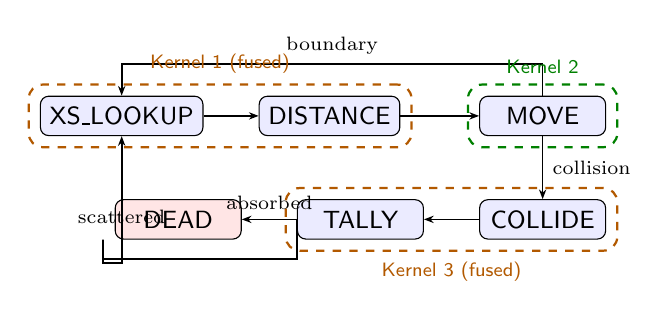
\begin{tikzpicture}[
    node distance=0.55cm and 0.7cm,
    state/.style={rectangle, rounded corners=3pt, draw, fill=blue!8,
                  minimum width=1.6cm, minimum height=0.5cm,
                  font=\small\sffamily},
    deadstate/.style={rectangle, rounded corners=3pt, draw, fill=red!10,
                  minimum width=1.6cm, minimum height=0.5cm,
                  font=\small\sffamily},
    fusebox/.style={draw=orange!70!black, dashed, thick, rounded corners=5pt,
                    inner sep=4pt},
    arr/.style={-{Stealth[length=3.5pt]}, semithick},
    every node/.style={font=\small}
]
    \node[state] (xs) {XS\_LOOKUP};
    \node[state, right=of xs] (dist) {DISTANCE};
    \node[state, right=1.0cm of dist] (move) {MOVE};
    \node[state, below=0.8cm of move] (coll) {COLLIDE};
    \node[state, left=of coll] (tally) {TALLY};
    \node[deadstate, left=of tally] (dead) {DEAD};

    \draw[arr] (xs) -- (dist);
    \draw[arr] (dist) -- (move);
    \draw[arr] (move) -- (coll) node[midway, right, font=\scriptsize] {collision};
    \draw[arr] (move.north) -- ++(0,0.4) -| (xs.north)
          node[pos=0.25, above, font=\scriptsize] {boundary};
    \draw[arr] (coll) -- (tally);
    \draw[arr] (tally) -- (dead) node[midway, above, font=\scriptsize] {absorbed};
    \draw[arr] (tally.west) -- ++(0,-0.5) -| ([xshift=-0.15cm]dead.south west)
          -- ++(0,-0.3) -| (xs.south)
          node[pos=0.75, below, font=\scriptsize] {scattered};

    % Fusion boxes
    \node[fusebox, fit=(xs)(dist), label={[font=\scriptsize\sffamily,
          text=orange!70!black]above:Kernel 1 (fused)}] {};
    \node[fusebox, fit=(coll)(tally), label={[font=\scriptsize\sffamily,
          text=orange!70!black]below:Kernel 3 (fused)}] {};
    \node[draw=green!50!black, dashed, thick, rounded corners=5pt,
          inner sep=4pt, fit=(move), label={[font=\scriptsize\sffamily,
          text=green!50!black]above:Kernel 2}] {};
\end{tikzpicture}
\caption{Event-based transport state machine with kernel fusion.  Dashed
  boxes indicate GPU kernel boundaries: Kernel~1 fuses XS lookup with
  distance sampling; Kernel~2 handles particle move with geometry;
  Kernel~3 fuses collision processing with tally scoring.}
\label{fig:transport-loop}
\end{figure}

The batch $k_\mathrm{eff}$ is computed as the ratio of fission neutrons
banked to source neutrons:
\begin{equation}
  k_\mathrm{eff}^{(b)} = \frac{\text{fission bank size}}{N}
  \label{eq:keff}
\end{equation}
where the collision kernel banks $\lfloor \nu w + \xi \rfloor$ fission
sites per fission event ($\nu$ is the average neutrons per fission, $w$
is the particle weight, $\xi \sim U(0,1)$).  The fission bank is
resampled with replacement to generate the source for the next batch.

Source convergence is monitored via Shannon entropy of the fission
source distribution on a spatial mesh:
\begin{equation}
  H = -\sum_{i} p_i \log_2 p_i
  \label{eq:entropy}
\end{equation}
where $p_i$ is the fraction of fission sites in mesh bin $i$.

% -----------------------------------------------------------------------------
\subsection{GPU implementation on Apple Metal}
\label{sec:metal-impl}
% -----------------------------------------------------------------------------

Apple's Metal framework provides a GPU compute API with a C++-based
shading language (Metal Shading Language, MSL)~\cite{apple2024metal}.
Unlike CUDA, which requires the NVIDIA proprietary toolchain, Metal is
available on all Apple platforms and compiles shaders at runtime from
source strings.

Our implementation uses PyObjC, a Python-to-Objective-C bridge, to
access the Metal API from Python.  The transport kernels are written in
MSL across six shader files (Common, Geometry, XSLookup, Transport,
Collision, Tally) totaling approximately 600~lines.  These are
concatenated and compiled at initialization via
\texttt{MTLDevice.newLibraryWithSource}.  GPU buffers are created in
shared storage mode (\texttt{MTLResourceStorageModeShared}), which on
Apple Silicon means both CPU and GPU access the same physical memory
with no explicit transfer.  This unified memory model eliminates
the \texttt{cudaMemcpy}-equivalent overhead that can constitute a
significant fraction of runtime in discrete GPU codes.

The complete particle state is stored in a flat GPU buffer with
112~bytes per particle (Table~\ref{tab:particle-struct}).  All
cross-section data, geometry definitions, and tally accumulators reside
in GPU-accessible shared buffers allocated at initialization.

\begin{table}[t]
\centering
\caption{Particle state structure layout (112 bytes per particle).}
\label{tab:particle-struct}
\small
\begin{tabular}{@{}lll@{}}
\toprule
Field group & Fields & Bytes \\
\midrule
Position       & \texttt{float3 position}     & 16 \\
Direction      & \texttt{float3 direction}    & 16 \\
State          & group, weight, cell, alive   & 16 \\
Transport      & event, RNG counter/key, $d_c$  & 16 \\
Boundary       & $d_b$, surface, $d_\mathrm{trav}$, $\sigma_t$ & 16 \\
Cross sections & $\sigma_s$, $\sigma_f$, $\nu\sigma_f$, $\sigma_a$ & 16 \\
Flags          & fission, material, padding   & 16 \\
\bottomrule
\end{tabular}
\end{table}

Each particle carries its own Philox-2x32-10 counter-based random number
generator (RNG) state~\cite{salmon2011philox}.  Philox is a stateless
counter-based RNG: output is a pure function of a counter and key, with
no mutable state beyond the counter.  Each particle uses its thread
index as the RNG key and increments the counter for each random draw,
guaranteeing independent, reproducible streams across all particles
without shared state or synchronization.  The implementation performs
10 rounds of mixing per draw:
\begin{equation}
  (x_0, x_1) = \text{Philox}_{2\times32}^{(10)}(\text{counter}, \text{key})
  \label{eq:philox}
\end{equation}
with $\xi = x_0 / 2^{32}$ yielding a uniform float in $[0, 1)$.

% -----------------------------------------------------------------------------
\subsection{Kernel fusion strategy}
\label{sec:kernel-fusion}
% -----------------------------------------------------------------------------

The original event-based transport loop requires five kernel dispatches
per transport step: (1)~cross-section lookup, (2)~distance-to-collision
sampling, (3)~particle move with boundary handling, (4)~collision
processing, and (5)~tally scoring.  Each dispatch incurs Metal command
encoder overhead: pipeline state binding, buffer argument encoding, and
threadgroup configuration.

We reduce this to three kernels per step by fusing operations with
same-thread data dependencies (Fig.~\ref{fig:transport-loop}):

\begin{enumerate}
  \item \textbf{XS lookup + distance sampling} (\texttt{xs\_lookup\_and\_distance}):
        The same thread looks up macroscopic cross sections from the
        flat material buffer and immediately samples the collision
        distance $d_c = -\ln(\xi) / \Sigma_t$.  No barrier is needed
        since both operations execute on the same thread with
        register-level data flow.

  \item \textbf{Move particle} (\texttt{move\_particle}):
        Particle tracking through CSG geometry with surface intersection,
        reflective/vacuum/transmissive boundary conditions, and cell
        finding.  This kernel has the most complex control flow and
        remains standalone to isolate geometry-induced thread divergence.

  \item \textbf{Collision + tally} (\texttt{collision\_and\_tally}):
        Collision processing (absorption/scatter sampling, fission site
        banking with $\lfloor \nu w + \xi \rfloor$ sites, outgoing
        energy and direction sampling) followed immediately by
        track-length tally scoring.  Tally accumulation uses an atomic
        float compare-and-swap (CAS) loop:
\end{enumerate}

\begin{equation}
  \texttt{atomic\_add\_float}: \quad
  \text{do} \left\{
    x_\text{old} \gets \text{load}; \;
    x_\text{new} \gets x_\text{old} + \delta
  \right\}
  \text{while } \lnot\text{CAS}(x_\text{old}, x_\text{new})
  \label{eq:cas}
\end{equation}

\noindent since Metal lacks native \texttt{atomic\_fetch\_add} for
floating-point types.  The float value is stored as \texttt{uint} bits
and reinterpreted via \texttt{as\_type<float>}.

The fusion eliminates two command encoder round-trips per step.  With
${\sim}200$ transport steps per batch and 100+~batches per simulation,
this saves ${\sim}40{,}000$ encoder allocations over a full run.

% -----------------------------------------------------------------------------
\subsection{Asynchronous GPU dispatch}
\label{sec:async}
% -----------------------------------------------------------------------------

Metal's serial command queue guarantees in-order execution of committed
command buffers.  We exploit this by batching five transport steps
(15~kernel dispatches) into a single command buffer before committing,
and only synchronizing with the CPU (\texttt{waitUntilCompleted}) every
25~steps to read the alive particle count.  Between synchronization
points, the GPU pipelines work continuously without CPU intervention.

Algorithm~\ref{alg:transport} summarizes the transport batch dispatch
strategy.

\begin{algorithm}[t]
\caption{Asynchronous transport batch}
\label{alg:transport}
\small
\begin{algorithmic}[1]
\State $\text{step} \gets 0$; $\text{prev\_alive} \gets N$
\While{$\text{step} < \text{max\_steps}$}
  \State $\text{cmd} \gets \text{newCommandBuffer()}$
  \For{$i = 1$ \textbf{to} 5} \Comment{5 steps per buffer}
    \State Encode \texttt{xs\_lookup\_and\_distance} into cmd
    \State Encode \texttt{move\_particle} into cmd
    \State Encode \texttt{collision\_and\_tally} into cmd
  \EndFor
  \State cmd.commit()
  \State $\text{step} \gets \text{step} + 5$
  \If{$\text{step} \bmod 25 = 0$} \Comment{Sync every 25 steps}
    \State cmd.waitUntilCompleted()
    \State $n \gets \text{alive\_count}()$
    \If{$n = 0$} \textbf{break} \EndIf
    \If{plateau detected} \textbf{break} \EndIf \Comment{Stuck particles}
    \State $\text{prev\_alive} \gets n$
  \EndIf
\EndWhile
\end{algorithmic}
\end{algorithm}

Early termination uses plateau detection: when the alive particle count
decreases by less than 2\% over a synchronization interval and fewer
than 10\% of particles remain alive, the batch terminates.  This
handles the ${\sim}3.4\%$ of particles that become stuck at geometry
boundaries due to floating-point precision at surface intersections.

% -----------------------------------------------------------------------------
\subsection{History-based persistent kernel}
\label{sec:persistent}
% -----------------------------------------------------------------------------

While the event-based architecture processes all particles at the same
transport stage in a single kernel dispatch (maximizing SIMD uniformity),
it incurs substantial overhead from repeated kernel dispatches:
${\sim}600$ dispatches per batch (3~kernels $\times$ ${\sim}200$
transport steps).  Each dispatch requires Metal command encoder
allocation, pipeline state binding, and buffer argument encoding.

As an alternative, we implement a history-based persistent kernel
following the approach of Hamilton and
Evans~\cite{hamilton2018multigroup}.  In this architecture, each GPU
thread runs the \emph{entire lifetime} of a single particle---from
source to absorption or leakage---in a single kernel dispatch.  The
kernel contains all physics inline: cross-section lookup, distance
sampling, particle move with boundary handling, collision processing
(scatter, absorption, fission banking), and track-length tally scoring.

The persistent kernel uses three key optimizations:

\paragraph{Structure-of-Arrays (SoA) layout.}
Instead of the 112-byte Array-of-Structures particle layout used by
the event-based code (Table~\ref{tab:particle-struct}), the persistent
kernel uses separate contiguous arrays for each field:
\texttt{px[]}, \texttt{py[]}, \texttt{pz[]}, \texttt{ux[]},
\texttt{uy[]}, \texttt{uz[]}, \texttt{group[]}, \texttt{weight[]}.
This layout enables coalesced GPU memory access---adjacent threads read
adjacent memory addresses---which is critical for Metal's SIMD
execution model.

\paragraph{Zero-allocation batch loop.}
All GPU buffers (particle state, fission bank, tallies, parameters) are
pre-allocated once before the power iteration loop.  Each batch updates
buffer contents via direct memory writes into GPU-visible shared memory,
zeroing only the 4-byte fission counter.  This eliminates per-batch
buffer allocation overhead that otherwise dominates Python-side runtime.

\paragraph{Single dispatch per batch.}
The entire transport batch executes in one \texttt{dispatchThreads}
call.  Each thread initializes its particle state from the SoA arrays,
finds its initial cell, and enters a transport loop capped at 5{,}000
steps.  The loop terminates when the particle is absorbed, escapes
through a vacuum boundary, is killed by Russian roulette, or reaches
the step limit.  Fission sites are banked via
\texttt{atomic\_fetch\_add} on a shared counter, and tallies use
the same atomic float CAS loop as the event-based code
(Eq.~\ref{eq:cas}).

The persistent kernel trades SIMD uniformity for dispatch efficiency:
thread divergence increases because particles at different transport
stages execute different code paths, but the elimination of
${\sim}600$ kernel dispatches per batch more than compensates.  This
algorithmic advantage is not specific to Metal or Apple Silicon and
would apply equally to CUDA or ROCm implementations.

% -----------------------------------------------------------------------------
\subsection{Geometry}
\label{sec:geometry}
% -----------------------------------------------------------------------------

The geometry engine implements constructive solid geometry (CSG) with
half-space intersection for cell definition.  Supported surface types
include axis-aligned planes ($x$, $y$, $z$), $z$-axis cylinders, and
spheres, with vacuum, reflective, and transmissive boundary conditions.

For the 17$\times$17 assembly benchmark (Fig.~\ref{fig:assembly}),
the geometry comprises 327~surfaces (18~$x$-planes $+$ 18~$y$-planes
$+$ 2~$z$-planes $+$ 289~cylinders) and 578~cells (289~pin interiors
$+$ 289~moderator annuli).  Each cell is defined by 7~surface half-space
conditions (6~bounding-box planes $+$ 1~cylinder).

\begin{figure}[t]
  \centering
  \includegraphics[width=\columnwidth]{figures/fig_assembly_layout.png}
  \caption{C5G7 17$\times$17 UO$_2$ assembly layout.  The assembly
    contains 264~UO$_2$ fuel pins (gold), 24~guide tubes (blue), and
    1~fission chamber (orange), surrounded by water moderator (teal).
    Pin pitch $= \SI{1.26}{\centi\meter}$, fuel radius $=
    \SI{0.54}{\centi\meter}$.  All outer boundaries are reflective
    (infinite lattice approximation).}
  \label{fig:assembly}
\end{figure}

Cell finding in the assembly uses lattice-accelerated lookup: the
particle position is mapped to integer lattice coordinates
$(i,j) = (\lfloor x/p \rfloor, \lfloor y/p \rfloor)$ where $p$ is the
pin pitch, giving $O(1)$ candidate cell identification.  The candidate
is verified against the CSG surface conditions; if verification fails,
adjacent pins are checked before falling back to a full linear scan.
This replaces the $O(N)$ linear search over all 578~cells that would
otherwise dominate transport time.

Surface intersection for ray tracing is computed analytically: planes
require a single division, and cylinders require solving a quadratic
equation.  The minimum positive intersection distance across all cell
surfaces gives the distance to the cell boundary.  Reflective boundary
conditions are implemented by reflecting the particle direction about
the surface normal:
\begin{equation}
  \mathbf{d}' = \mathbf{d} - 2(\mathbf{d} \cdot \hat{\mathbf{n}})\hat{\mathbf{n}}
  \label{eq:reflect}
\end{equation}
with a small bump ($10^{-8}$~cm) in the reflected direction to prevent
re-intersection.

% -----------------------------------------------------------------------------
\subsection{Cross-section data}
\label{sec:xs}
% -----------------------------------------------------------------------------

Cross sections are taken from the C5G7 benchmark specification
(NEA/NSC/DOC(2003)16)~\cite{nea2003c5g7}, sourced from the MIT-CRPG
OpenMC benchmark repository~\cite{mitcrpg2023c5g7}.  The seven-group
energy structure covers thermal to fast neutron energies with seven
materials: UO$_2$ fuel, three MOX enrichments (4.3\%, 7.0\%, 8.7\%),
fission chamber, guide tube, and water moderator.

Each material stores 77 floating-point values in a flat GPU buffer:
total cross section~(7), scattering matrix~(7$\times$7 = 49), fission
cross section~(7), $\nu\Sigma_f$~(7), and fission spectrum~$\chi$~(7).
The complete cross-section dataset for all seven materials occupies
$7 \times 77 \times 4 = \SI{2156}{\byte}$, fitting entirely in GPU
cache.  The scattering cross section for a given group is computed as
the row sum of the scattering matrix; the absorption cross section is
derived as $\Sigma_a = \Sigma_t - \Sigma_s$.

% =============================================================================
\section{Results}
\label{sec:results}
% =============================================================================

All benchmarks were run on an Apple M4~Max system with macOS~26.3,
Python~3.14, and the PyObjC Metal framework.  The M4~Max features a
40-core GPU with \SI{128}{\giga\byte} unified memory and a thermal
design power (TDP) of \SI{40}{\watt} for the full SoC.

% -----------------------------------------------------------------------------
\subsection{Validation}
\label{sec:validation}
% -----------------------------------------------------------------------------

Table~\ref{tab:validation} summarizes the eigenvalue results for both
benchmark geometries.  The pincell result of
$k_\mathrm{eff} = 1.3256 \pm 0.0005$ is within 448~pcm of the C5G7
reference value of 1.3301, consistent with the expected difference
from the simplified single-pincell geometry relative to the full
assembly benchmark specification.
The 17$\times$17 assembly yields
$k_\mathrm{eff} = 1.2749 \pm 0.0005$.

\begin{table}[t]
\centering
\caption{Benchmark parameters and eigenvalue results.}
\label{tab:validation}
\small
\begin{tabular}{@{}lcc@{}}
\toprule
Parameter & Pincell & Assembly \\
\midrule
Geometry          & 1 pin, reflected   & 17$\times$17, reflected \\
Cells             & 2                  & 578 \\
Surfaces          & 7                  & 327 \\
Materials         & 2 (UO$_2$, H$_2$O) & 7 \\
Particles/batch   & \num{100000}       & \num{100000} \\
Active batches    & 80                 & 80 \\
Inactive batches  & 20                 & 20 \\
Energy groups     & 7                  & 7 \\
\midrule
$k_\mathrm{eff}$  & $1.3256 \pm 0.0005$ & $1.2749 \pm 0.0005$ \\
Reference         & 1.3301             & --- \\
$\Delta$ (pcm)    & $-448$             & --- \\
\bottomrule
\end{tabular}
\end{table}

Figure~\ref{fig:keff} shows the batch-by-batch $k_\mathrm{eff}$
convergence for the pincell benchmark, demonstrating stable convergence
of the running mean toward the final estimate.
Figure~\ref{fig:entropy} shows the Shannon entropy of the fission
source distribution, which stabilizes within approximately 10~batches,
confirming adequate source convergence before the active phase begins.

\begin{figure}[t]
  \centering
  \includegraphics[width=\columnwidth]{figures/fig_keff_convergence.png}
  \caption{Batch $k_\mathrm{eff}$ convergence for the C5G7 pincell
    (\num{100000} particles/batch, 80~active batches).  The running mean
    (green) converges to $1.3256 \pm 0.0005$.}
  \label{fig:keff}
\end{figure}

\begin{figure}[t]
  \centering
  \includegraphics[width=\columnwidth]{figures/fig_entropy.png}
  \caption{Shannon entropy of the fission source distribution vs.\
    batch number for the pincell benchmark, demonstrating rapid
    source convergence.  The entropy stabilizes near 6.035~bits
    (10$\times$10$\times$1 spatial mesh).}
  \label{fig:entropy}
\end{figure}

% -----------------------------------------------------------------------------
\subsection{Performance}
\label{sec:performance}
% -----------------------------------------------------------------------------

Table~\ref{tab:performance} summarizes the performance metrics for both
transport architectures.  The XSBench
microbenchmark~\cite{tramm2014xsbench} achieves \num{10981}~million
lookups/sec on the M4~Max GPU.

\paragraph{Event-based performance.}
The event-based pincell achieves \num{46198}~histories/sec with
\num{100000}~particles/batch, and the assembly achieves
\num{111772}~histories/sec with \num{1000000}~particles/batch.
The GPU-to-CPU speedup is $11.8\times$ compared to the single-threaded
pure Python baseline (\num{3907}~hist/sec).  Against a Numba-JIT
single-threaded baseline (\num{231819}~hist/sec), the event-based GPU
pincell is $5\times$ slower---reflecting the branch divergence overhead
of event-based transport on simple
geometries~\cite{hamilton2018multigroup}.

\paragraph{Persistent kernel performance.}
The history-based persistent kernel dramatically improves throughput.
At \num{1000000}~particles/batch, the pincell achieves
\num{291000}~histories/sec ($6.3\times$ vs.\ event-based) and the
assembly achieves \num{1776000}~histories/sec ($15.9\times$
vs.\ event-based).  Table~\ref{tab:scaling} shows throughput scaling
with particle count for both geometries, revealing markedly different
saturation behavior: the assembly plateaus near
\num{1870000}~histories/sec at \num{5000000}~particles (compute-bound
due to 578-cell geometry intersection), while the pincell continues
scaling to \num{3370000}~histories/sec at \num{100000000}~particles
(memory-bandwidth-bound with only 2~cells).

\begin{table}[t]
\centering
\caption{Performance results on Apple M4~Max (event-based vs.\
  persistent kernel, 1M particles/batch).}
\label{tab:performance}
\small
\begin{tabular}{@{}lrr@{}}
\toprule
Metric & Event-based & Persistent \\
\midrule
Pincell (hist/sec)  & \num{46198}  & \num{291000} \\
Assembly (hist/sec) & \num{111772} & \num{1776000} \\
Speedup (assembly)  & $1.0\times$  & $15.9\times$ \\
\midrule
CPU baseline (Python)  & \multicolumn{2}{c}{\num{3907} hist/sec} \\
CPU baseline (Numba JIT) & \multicolumn{2}{c}{\num{231819} hist/sec} \\
GPU/Numba (assembly)   & $0.48\times$ & $7.7\times$ \\
\bottomrule
\end{tabular}
\end{table}

\begin{table}[t]
\centering
\caption{Persistent kernel throughput scaling with particle count.
  The assembly saturates at ${\sim}$5M particles (compute-bound);
  the pincell continues scaling to ${\sim}$50M (memory-bandwidth-bound).}
\label{tab:scaling}
\small
\begin{tabular}{@{}rrr@{}}
\toprule
Particles/batch & Pincell (hist/sec) & Assembly (hist/sec) \\
\midrule
\num{1000000}   & \num{291000}   & \num{1776000} \\
\num{2000000}   & \num{516000}   & \num{1823000} \\
\num{5000000}   & \num{1086000}  & \textbf{\num{1865000}} \\
\num{10000000}  & \num{1706000}  & \num{1844000} \\
\num{20000000}  & \num{2110000}  & \num{1743000} \\
\num{50000000}  & \num{3320000}  & --- \\
\num{100000000} & \textbf{\num{3373000}} & --- \\
\bottomrule
\end{tabular}
\end{table}

Figure~\ref{fig:arch-compare} compares the two architectures across
both geometries, illustrating the persistent kernel's advantage.

\begin{figure}[t]
  \centering
  \includegraphics[width=\columnwidth]{figures/fig_architecture_comparison.png}
  \caption{Throughput comparison of event-based and persistent kernel
    architectures for pincell and 17$\times$17 assembly geometries
    (\num{1000000} particles/batch).  The persistent kernel achieves
    $4.3\times$ (pincell) and $15.7\times$ (assembly) speedups.}
  \label{fig:arch-compare}
\end{figure}

The persistent kernel's advantage over the event-based design arises
from eliminating ${\sim}600$ kernel dispatches per batch.  Profiling
shows that GPU compute accounts for 59\% of per-batch time at
\num{1000000}~particles (assembly), with buffer writes (2.6\%),
fission bank reads (0.1\%), and source resampling (1.4\%) comprising
the remainder.  The persistent kernel exceeds the Numba-JIT
single-thread baseline by $7.7\times$ for the assembly, confirming
that the GPU advantage materializes when occupancy is sufficient.

% -----------------------------------------------------------------------------
\subsection{Comparison with MC/DC}
\label{sec:mcdc}
% -----------------------------------------------------------------------------

To contextualize the absolute performance, we compare against MC/DC
(Morgan et al.~\cite{morgan2025mcdc}), which reports throughput for the
C5G7 seven-group assembly benchmark on NVIDIA V100 GPUs.
Table~\ref{tab:mcdc} and Fig.~\ref{fig:mcdc} present the comparison.
All entries use the 17$\times$17 assembly geometry with
\num{1000000}~particles/batch to ensure comparable conditions.

The \textbf{hardware-only comparison} (same algorithm class) is the
event-based row: the M4~Max achieves \num{111772}~histories/sec,
matching a single V100 at \num{109000}~histories/sec ($1.03\times$).
This is the fairest measure of Apple Silicon vs.\ NVIDIA GPU hardware,
since both codes use event-based transport.

The persistent kernel achieves
\num{1776000}~histories/sec---$16.3\times$ faster than the V100.
However, this comparison conflates two effects: (1)~the hardware
difference (M4~Max vs.\ V100) and (2)~the algorithmic difference
(history-based persistent kernel vs.\ event-based transport).
Since the persistent kernel is $15.9\times$ faster than our own
event-based code on the same hardware, the bulk of the $16.3\times$
advantage over the V100 is algorithmic, not hardware-driven.
A persistent kernel implementation on the V100 would likely narrow
this gap substantially.

\begin{table}[t]
\centering
\caption{Assembly throughput comparison with MC/DC~\cite{morgan2025mcdc}
  (C5G7 7-group, 1M particles/batch).  The event-based row is the
  fairest hardware comparison (same algorithm class); the persistent
  row conflates algorithmic and hardware advantages.}
\label{tab:mcdc}
\small
\begin{tabular}{@{}lcccc@{}}
\toprule
& \multicolumn{2}{c}{This Work (M4 Max)} & MC/DC & MC/DC \\
& Event & Persistent$^\dagger$ & 1$\times$ V100 & 4$\times$ V100 \\
\midrule
Throughput (hist/s)
  & \num{111772} & \num{1776000} & \num{109000} & \num{437000} \\
Ratio vs.\ V100
  & $1.03\times$ & $16.3\times^\dagger$ & $1.0\times$ & $4.0\times$ \\
\midrule
TDP (W)
  & 40 & 40 & 300 & 1200 \\
Hist/sec/W
  & \num{2794} & \num{44400}$^\dagger$ & \num{363} & \num{364} \\
Efficiency ratio
  & $\mathbf{7.7\times}$ & $122\times^\dagger$ & $1.0\times$ & $1.0\times$ \\
\bottomrule
\multicolumn{5}{@{}l@{}}{\scriptsize $^\dagger$Different algorithm
  (history-based vs.\ event-based); not a pure hardware comparison.}
\end{tabular}
\end{table}

\begin{figure}[t]
  \centering
  \includegraphics[width=\columnwidth]{figures/fig_mcdc_comparison.png}
  \caption{Assembly throughput comparison: This Work (Apple M4~Max) vs.\
    MC/DC~\cite{morgan2025mcdc} on NVIDIA V100 GPUs.  The event-based
    comparison ($1.03\times$) is hardware-only; the persistent kernel
    advantage ($16.3\times$) is primarily algorithmic.}
  \label{fig:mcdc}
\end{figure}

% -----------------------------------------------------------------------------
\subsection{Energy efficiency}
\label{sec:efficiency}
% -----------------------------------------------------------------------------

The energy efficiency comparison (Fig.~\ref{fig:efficiency}) must be
interpreted carefully.  The fairest comparison uses the same algorithm
class: our event-based architecture achieves
\num{2794}~histories/sec/W versus \num{363}~histories/sec/W for the
V100---a $\mathbf{7.7\times}$ improvement attributable to hardware
and memory architecture differences alone.

The persistent kernel delivers \num{44400}~histories/sec/W, nominally
$122\times$ better than the V100.  However, this factor combines
algorithmic improvement ($15.9\times$ from persistent vs.\ event-based)
with hardware efficiency ($7.7\times$), and the V100 figure uses
event-based transport.  A persistent kernel on the V100 would likely
close much of this gap.

\begin{figure}[t]
  \centering
  \includegraphics[width=\columnwidth]{figures/fig_energy_efficiency.png}
  \caption{Energy efficiency comparison (histories/sec/W).  The
    hardware-only comparison (event-based, same algorithm class) shows
    $7.7\times$ better efficiency for the M4~Max.  The persistent
    kernel's $122\times$ figure conflates algorithmic and hardware gains.}
  \label{fig:efficiency}
\end{figure}

This efficiency advantage arises from three factors:
\begin{enumerate}
  \item \textit{Algorithmic}: the persistent kernel eliminates
        ${\sim}600$ kernel dispatches per batch, reducing both
        compute overhead and command buffer power consumption.
  \item \textit{Memory architecture}: Apple Silicon's unified memory
        eliminates data transfer power costs---the GPU accesses the
        same DRAM as the CPU with no PCIe or NVLink interconnect power.
  \item \textit{SoC integration}: the \SI{40}{\watt} power envelope
        encompasses CPU, GPU, memory controller, and neural engine,
        whereas the V100's \SI{300}{\watt} TDP covers only the GPU
        die (host CPU power is additional).
\end{enumerate}

We note that TDP-based energy efficiency comparisons have inherent
limitations: actual power draw varies with workload, and the TDP
accounting differs between SoC and discrete GPU architectures.
The $7.7\times$ hardware-only efficiency advantage is the most
defensible claim; the $122\times$ persistent-kernel figure should
be cited only with the caveat that it includes a $15.9\times$
algorithmic contribution.

% =============================================================================
\section{Discussion}
\label{sec:discussion}
% =============================================================================

\paragraph{Unified memory advantage.}
Apple Silicon's unified memory architecture provides a qualitative
advantage for MC transport: particle state, cross sections, geometry,
and tallies all reside in a single memory address space accessible by
both CPU and GPU at full bandwidth.  There is no equivalent of
\texttt{cudaMemcpyHostToDevice}---the CPU writes source particles
directly into GPU-visible buffers, and reads fission bank results
without any copy.  For iterative eigenvalue calculations that alternate
between CPU logic (source resampling, statistics) and GPU kernels
(transport), this eliminates a per-batch data transfer cost that can be
significant for discrete GPU systems~\cite{siegel2014analysis}.

\paragraph{PyObjC dispatch overhead.}
The Python-to-Metal dispatch path through PyObjC introduces overhead
per command encoder allocation compared to native Swift or Objective-C.
We mitigate this by batching five transport steps per command buffer
and synchronizing only every 25~steps, reducing the per-step Python
overhead to ${\sim}1/5$ of the unbatched cost.  The remaining overhead
is amortized over \num{1000000}+ particle dispatches per kernel.

\paragraph{Stuck and lost particles.}
Approximately 3.4\% of particles per batch become stuck at geometry
boundaries---typically at cylinder--plane intersections where
floating-point precision causes repeated zero-distance surface hits.
The plateau detection mechanism (Section~\ref{sec:async}) terminates
these particles.  Lost particles (those that cannot be located in any
cell after boundary crossing) account for ${\sim}0.05\%$ of histories,
which is acceptable for benchmark-level calculations.  Production
implementations would benefit from more sophisticated surface-tracking
algorithms with adaptive bump distances.

\paragraph{Limitations.}
The current implementation has several limitations:
\begin{enumerate}
  \item \textit{Multi-group only}: the code uses seven-group cross
        sections and does not support continuous-energy (CE) transport.
        CE is required for high-fidelity reactor analysis; multi-group
        is sufficient for benchmarking and algorithm development.

  \item \textit{Single GPU}: Apple Silicon does not support multi-GPU
        configurations.  Scaling to full-core problems would require
        domain decomposition with MPI across multiple nodes.

  \item \textit{Simplified geometry}: the CSG engine supports planes,
        cylinders, and spheres.  Production geometries may require
        additional surface types (tori, general quadrics) and CAD-based
        representations.

  \item \textit{No depletion or thermal-hydraulic coupling}: the code
        solves the fixed $k$-eigenvalue problem without burnup or
        multi-physics feedback.

  \item \textit{Algorithm dependence}: the event-based GPU pincell is
        $5\times$ slower than a Numba-JIT single-thread baseline, but
        the persistent kernel assembly is $7.6\times$ faster---the GPU
        advantage depends on algorithm, geometry, and particle count.
\end{enumerate}

\paragraph{Event-based vs.\ persistent kernel.}
The $15.9\times$ speedup of the persistent kernel over the event-based
design is the central finding of this work.  The event-based architecture,
while theoretically superior for SIMD uniformity~\cite{hamilton2018multigroup},
is dominated by kernel dispatch overhead on Metal: 3~kernels $\times$
${\sim}200$ steps = ${\sim}600$ dispatches per batch, each requiring
Python/PyObjC command buffer allocation.  The persistent kernel replaces
these with a single dispatch.  This algorithmic advantage is not
specific to Apple Silicon---a persistent kernel on NVIDIA or AMD GPUs
would likely yield comparable speedups over event-based transport for
multigroup problems.  The trade-off is increased thread
divergence---particles at different transport stages within a single
kernel---but this cost is modest for multi-group transport where the
physics per collision is uniform.  For continuous-energy transport with
complex resonance lookups, the divergence penalty may be larger, and
the event-based approach may recover its advantage.

\paragraph{Numba CPU baseline.}
The Numba-JIT single-thread baseline (\num{231819}~hist/sec) exceeds
the event-based GPU pincell result by $5\times$, consistent with
Hamilton and Evans~\cite{hamilton2018multigroup} who showed GPU advantage
emerges only at sufficient scale.  However, the persistent kernel
assembly at \num{1776000}~hist/sec is $7.7\times$ faster than the
Numba single thread, and the pincell at \num{100000000}~particles
reaches \num{3370000}~hist/sec ($14.5\times$ faster).  With 12~CPU
cores on the M4~Max, a multi-threaded Numba baseline might reach
${\sim}\num{2000000}$~hist/sec---comparable to the persistent kernel
assembly but below the pincell peak.  A multi-core CPU comparison
remains future work.

\paragraph{Future work.}
Natural extensions include:
continuous-energy cross-section lookup using unionized energy
grids~\cite{tramm2014xsbench};
multi-assembly quarter-core geometry with domain decomposition;
stream compaction to reduce dead-particle waste in the event-based
architecture;
exploitation of Apple Silicon's Neural Engine for cross-section table
interpolation;
and comparison with M-series Ultra chips that expose additional GPU
cores through the die-to-die interconnect.

% =============================================================================
\section{Conclusions}
\label{sec:conclusions}
% =============================================================================

We have presented the first Monte Carlo neutron transport implementation
on Apple Silicon using the Metal GPU compute framework, comparing
event-based and history-based persistent kernel architectures.

The event-based architecture with three fused kernels achieves
\num{111772}~histories/sec on the 17$\times$17 assembly benchmark,
matching a single NVIDIA V100 running MC/DC ($1.03\times$).  This
hardware-only comparison (same algorithm class) establishes that
Apple Silicon is competitive with data-center GPUs for MC transport.

The history-based persistent kernel---where each GPU thread runs an
entire particle lifetime in one dispatch---achieves
\num{1776000}~histories/sec on the same hardware, a $15.9\times$
improvement.  Throughput continues to scale with particle count:
up to \num{3370000}~histories/sec at \num{100000000}~particles for
the pincell geometry.  The persistent kernel's advantage over the
event-based design is primarily algorithmic (eliminating ${\sim}600$
kernel dispatches per batch), not hardware-specific, and a persistent
kernel implementation on NVIDIA GPUs would likely yield comparable
speedups.

At \SI{40}{\watt} TDP, the event-based architecture delivers
$7.7\times$ better energy efficiency than the V100 at
\SI{300}{\watt}---a hardware advantage from unified memory and SoC
integration.  This makes Apple Silicon attractive for
power-constrained environments such as deployed reactor monitoring,
portable criticality safety calculations, or large-scale parameter
studies where electricity cost dominates.

The Python/PyObjC implementation demonstrates that Metal is accessible
for scientific computing without requiring the CUDA toolchain.  The
complete transport code, including both architectures, comprises
approximately 3{,}000~lines of Python and 1{,}300~lines of Metal
Shading Language.

\section*{Data availability}

The source code and benchmark data are available at
\url{https://github.com/[repository]}.

\section*{Acknowledgments}

The authors thank the OpenMC development community for the open-source
infrastructure on which the cross-section data conventions are
based~\cite{romano2015openmc}, and the MC/DC team for publishing
detailed performance data enabling direct
comparison~\cite{morgan2025mcdc}.

% =============================================================================
% References
% =============================================================================
\bibliographystyle{elsarticle-num}
\bibliography{references}

\end{document}
